% Chapter Template

\chapter{Solution Design} % Main chapter title

\label{ChapterX} % Change X to a consecutive number; for referencing this chapter elsewhere, use \ref{ChapterX}

\section{General Approach} \label{sec:generalApproach}

With the purpose of enabling the execution of software engineering tasks at APK level, we propose a three phase process depicted in Figure \ref{fig:proposeApproach}. The first phase consists of APK processing in order to generate models of the application, and the second phase consists of using those models by a certain module that represent a software engineering task desired by users. The final phase consists in rebuilding the APK when required, as in the case of mutation testing or app instrumentation for dynamic analysis. Note that enabling automated software engineering tasks at APK level is our long term goal, therefore, rebuilding the APK (but whitout decompiling the app to get the source code) is a required step in our approach.

\begin{figure}[htbp]
	\centerline{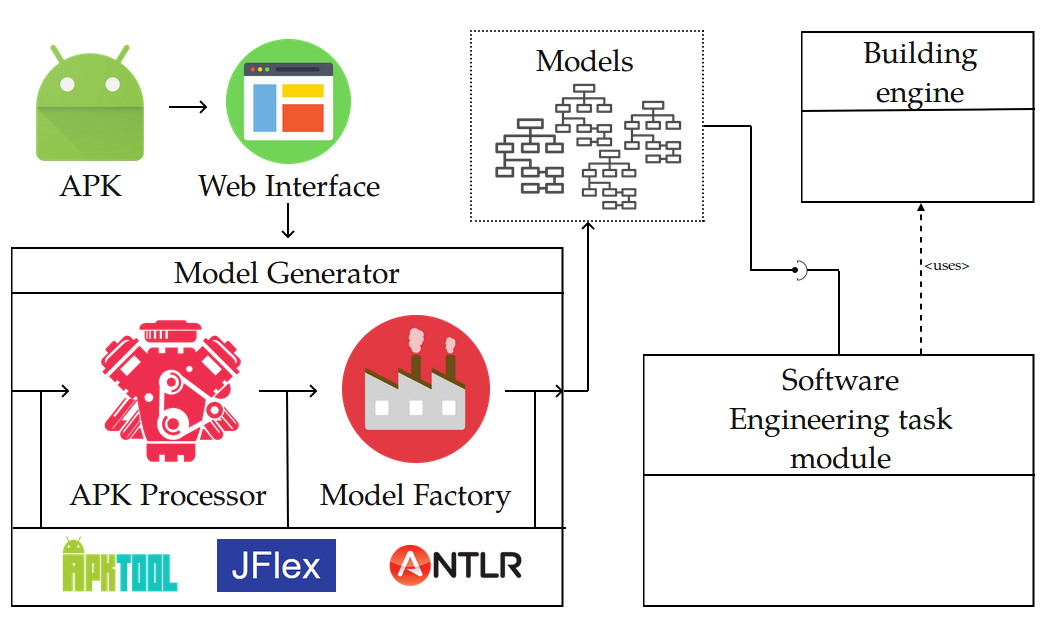
\includegraphics[width=0.9\textwidth]{Figures/proposedApproach.png}}
	\caption{Architecture of the proposed approach}
	\label{fig:proposeApproach}
\end{figure}

\textbf{APK processing.} The first step during the model generation is  decoding an APK file to be able to extract the Android opcodes and resources. Note that an APK is a zip file that contains resources files and a classes file that include the opcodes in DEX format for all the classes belonging to an Android app (including libraries). Based on the wide usage of SMALI as intermediate representation (top 2 according to Li \textit{et. al.,} \cite{li:IST2017}) and that it keeps about 97\% of the information in an APK  \cite{arnatovich2014empirical,arnatovich2018comparison}, we propose it as the representation used for the models extraction. There are already parsers and lexers for SMALI which allows the extraction of abstract syntax trees (ASTs). Concerning the textual information available in resources files, it can be easily extracted because of the XML nature of those files in Android. Note that extracting SMALI code does not require de-compilation to original source code (\textit{e.g.,} Java) which is time consuming and prone to de-compilation errors.

\textbf{Software Engineering Tasks modules.} Because SMALI can be used to extract representations and models such as ASTs, control flow graphs, among others, a plethora of analysis can be instantiated and without the need of original source code. Given the models of the application, implementing a software engineering task must be done on a separate module. These modules must be able to consume the models and provide a comprehensive result to the user. For example, a mutation testing module at APK level must use the AST models extracted from SMALI code to (i) identify the possible mutable snippets of code, and (ii) mutate the original app.


\textbf{Re-building/packaging the app}.
The last phase of this process, consist of going back from decoded SMALI representation to an executable APK file, which does not require recompiling the modified code. However, note that this requires to be very careful when modifying the SMALI code to avoid injecting bugs into the app when the SMALI syntax is not properly used.%For this, we propose to use of APKTool \textit{build} function that from a SMALI representation of an app allows to build an APK. 
This building process must be called by each software engineering task module, making sure all modules that require the execution of this process use the same format to deliver the internal result.



\section{MutAPK}

In order to validate the feasibility of our proposed approach we decided to implement it using mutation testing as a reference. As it was shown in the Section 3, mutation testing is still one of the software engineering tasks that has not been developed at APK level. Consequently, we implemented the proposed approach in a tool ( \textit{\textbf{MutAPK}} ) that allowed us to compare the obtained results when working in the scenarios of having source code, and having only APK files.

As it was mention before, MutAPK must comply to some must-have rules for all mutation testing tools, it has a set of mutant operators, it provides the possibility to select the mutant operators that will be executed, it defines in detail the short process required for its extension and enables parallel execution. MutAPK is an Open Source project available at \url{https://github.com/TheSoftwareDesignLab/MutAPK}. In the following sections, we describe MutAPK according to its workflow described in Figure \ref{fig:mutapkArchitecture}

\begin{figure}[htbp]
	\centerline{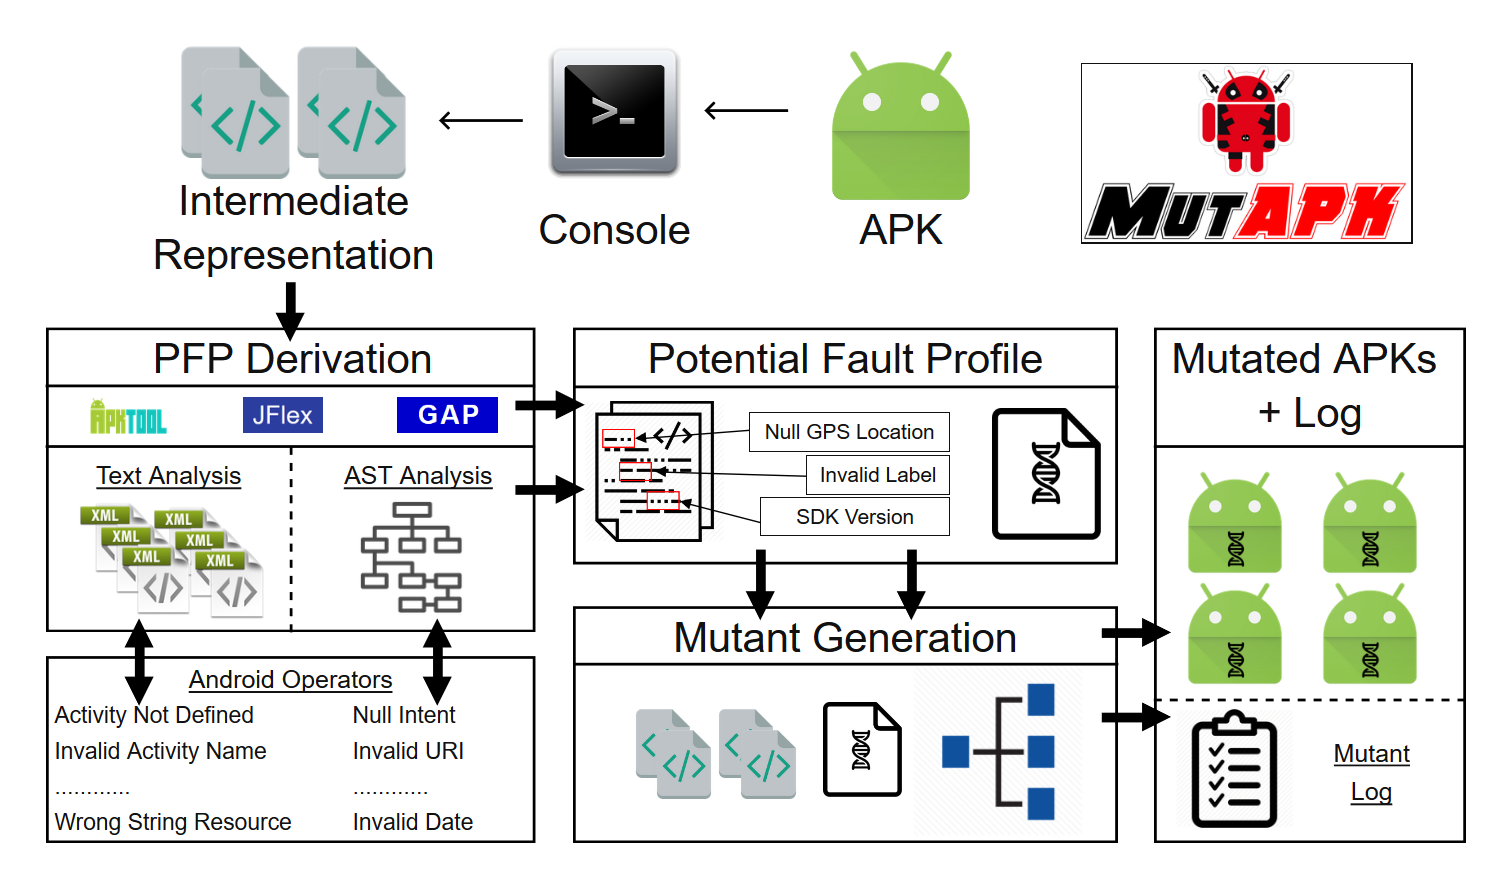
\includegraphics[width=0.9\textwidth]{Figures/mutapkArchitecture.png}}
	\caption{Architecture of MutAPK}
	\label{fig:mutapkArchitecture}
\end{figure}

\subsection{APK Processing}
\subsubsection{Unpackaging/Packaging APK}

Recalling the study by Arnatovich \textit{et al.} \cite{arnatovich2018comparison}, we use APKTool, which allows us to process an APK returning a folder with all the resource files decoded and the source files disassembled into SMALI files. Additionally, code-related files are presented in a useful project like file structure. Because of this, some source code analysis tasks that are based in file location can be easily translated to be executed over APKTool decoding result. At the same time, APKTool allows to build an unsigned apk from the previously mention files. Therefore, an application can be modified in its SMALI representation and then packaged again into an APK for its use.

\subsubsection{Derivation of the Potential Fault Profile}

We followed the same approach proposed by Linares-V\'asquez \emph{et al.} \cite{linares2017enabling,Moran:ICSE18} Therefore, we detect mutation locations by extracting a Potential Fault Profile, and then we implement mutation operations on those locations. The \textit{\textbf{P}otential \textbf{F}ault \textbf{P}rofile \textbf{PFP}} is a set of code locations that represent potential points were a fault can be injected. These potential fault injection points are defined through the mutation operators shown in the Section \ref{sssec:imo}. For the implementation of MutAPK, the PFP definition was inherited from MDroid+. First, both XML and SMALI files are statically analyzed searching for instructions that comply with the characteristics defined in the mutation operators. This previous process, also inherited from MDroid+, consist for XML files of going through the content looking for matches between the file tags and the different mutation operators potential fault injection points. 

On the other hand, for SMALI files the process is based on the Abstract Syntax Tree that is obtained using the lexer and parser created by APKTool to perform the disassembling of an APK. In particular, MutAPK uses the visitor design pattern  to identify the possible locations. Knowing this, the process can easily be extended to add new operators and to provide more comprehensive analysis of the app (\textit{i.e.,} resource and SMALI files) if needed. The final result of the PFP derivation process is a list that joins the potential fault injection points with the mutation operators that can be applied to those locations.
\subsection{Mutation Testing Module}
\subsubsection{Operators}
\label{sssec:imo}
We built upon the 38 operators proposed by  Linares-V\'asquez \emph{et al.} \cite{linares2017enabling,Moran:ICSE18} , which are representative of  potential fault in Android apps and  can be found either on  source code statements, XML tags, or locations in other resource files. In MutAPK we implemented (i) the 33 operators implemented in MDroid+ that do not lead to compilation errors, and (ii) two additional operators not available in MDroid+.

 
Therefore, our work was to translate the  operators implementation from the original source code-based implementations to the corresponding implementations in the SMALI representation. In order to do this, we manually selected 11 apps that had potential locations for implementing the operators. Given those applications, we built the APKs using Android Studio and disassembled manually each one to recognize the direct translation of each mutation original statement. After this dictionary is created, we proceeded to mutate manually the source code of these 11 applications and proceed to generate again the APK files. Finally we performed a diff comparison between the SMALI representation of the original version against the SMALI representation of the mutated version. Because of this, we were able to translate successfully each mutation operator from source code to SMALI representation. With this procedure we derived the list of operators implementation at APK level; the details of each operator are available in our online appendix \cite{MutAPK}.

\subsubsection{Mutant Creation}

We start by unpackaging the apk into a temporal folder. After that, the PFP is derived and a list of potential fault injection locations is created. We now can use the defined mutation rules to generate the mutants, however, in order to make this process as efficiently as possible, MutAPK provides the option to parallelize the mutant creation. For each location in the PFP, a copy of the disassembled apk is created. After the copying ends, based on the mutation operator associated, a new process that translate the mutation rule into an actual change is executed over the exact location inside the associated folder. Next, a compilation process is triggered in order to generate as result an APK. As it was said before, this process can be parallelized and each task consist of: copying the dissambled apk, mutating either a resource file or a SMALI file, and finally compiling the result to obtain an APK.  Nota that while MDroid+ only generates the source code of the mutants, MutAPK is able to generate APKs ready to install and test.

\subsubsection{Extensibility}

Due to the fast change of the android framework, MutAPK must provide the possibility to add new mutation operators easily. Therefore, in order to enable a new mutation operator some changes must be implemented: (i) create a new detector/locator that is capable of finding the correct position that provides all the information needed to create a \textit{Mutation Location} defined in MutAPK; (ii) a mutator, that is capable of using the previously identified location information to mutate the code or resource file; (iii) update the \textit{operator-types.properties} file found under the "src/uniandes/tsdl/mutapk" folder to add the new mutation operator file path with its defined id; (iv) modify \textit{OperatorBundle.java} (in case the new operator is text-based) to add the new text detector and (v) update the \textit{operators.properties} file.

At the same time, MutAPK counts with an \textit{extra} folder where the external libraries are located. Therefore, if user wants to improve the file analysis process or wants to execute a more specialized process over the application, he can save the library files in this folder and manage them easily. MutAPK has in this \textit{extra} folder the \textit{jar} file provided by APKTool. Note that here there is a big difference with MDroid+ implementation; because in MDroid+ the source code must be compiled, then it requires in the extra folder all the libraries required to compile the source, code. This is not required in MutAPK because we are already working with "compiled" code.
\subsection{Tool Usage}
MutAPK has been designed to work as a command line tool. In order to use it, the user must have installed Maven and Java. The MutAPK repository\cite{MutAPK} must be cloned and then packaged using the following commands

\begin{minipage}{\linewidth}
	\begin{lstlisting}[language={sh}, label={lst:mvn}, caption={Git and Maven commands to build MutAPK}, numbers=none]
git clone https://github.com/TheSoftwareDesignLab/MutAPK.git
mvn clean
mvn package
	\end{lstlisting}
\end{minipage}\\

After that, the  jar file called MutAPK-<version>.jar will be located in the \textit{target} folder. That file can be relocated and used in other places. 

\begin{minipage}{\linewidth}
	\begin{lstlisting}[language={sh}, label={lst:ccrM}, caption={Console command to run MutAPK}, numbers=none]
java -jar MutAPK-<version>.jar <APKPath> <AppPackage> <OutputFolder> <ExtraComponentFolder> <operatorsDir> <multithread>
	\end{lstlisting}
\end{minipage}\\

To run it, the previous command must be used (Listing \ref{lst:ccrM}),  where
\begin{enumerate}
	\item \textbf{<APKPath>} is the path to the app's APK
	\item \textbf{<APKPackage>} is the app package used to identify the code that belongs to the app (not the libraries)
	\item \textbf{<OutputFolder>} is the path to the folder where all the mutants will be generated.
	\item \textbf{<ExtraComponentFolder>} is the path to the folder that has the extra libraries used by MutAPK
	\item \textbf{<operatorsDir>} is the path to the \textit{operators.properties} folder, that describes the operators that must be used to generate mutants
	\item \textbf{<multithread>} boolean value, defines if MutAPK must be executed using multiple threads
\end{enumerate}
\begin{minipage}{\textwidth}
	\begin{lstlisting}[language={sh}, label={lst:eompa}, caption={Example Output of MutAPK for PhotoStream app}, numbers=none]
Amount Mutants	Mutation Operator
1		OOM_LARGE_IMAGE
3		NULL_INTENT
5		NULL_OUTPUT_STREAM
1		INVALID_FILE_PATH
5		INVALID_LABEL
19		NULL_VALUE_INTENT_PUT_EXTRA
7		INVALID_COLOR
9		FINDVIEWBYID_RETURNS_NULL
19		INVALID_KEY_INTENT_PUT_EXTRA
5		LENGTHY_GUI_CREATION
8		VIEW_COMPONENT_NOT_VISIBLE
3		NULL_INPUT_STREAM
0		SDK_VERSION
7		INVALID_ACTIVITY_PATH
8		INVALID_VIEW_FOCUS
2		CLOSING_NULL_CURSOR
39		WRONG_STRING_RESOURCE
3		WRONG_MAIN_ACTIVITY
1072		NULL_METHOD_CALL_ARGUMENT
4		NULL_BACKEND_SERVICE_RETURN
2		LENGTHY_GUI_LISTENER
9		INVALID_ID_FINDVIEW
7		ACTIVITY_NOT_DEFINED
5		MISSING_PERMISSION_MANIFEST
2		LENGTHY_BACKEND_SERVICE
3		DIFFERENT_ACTIVITY_INTENT_DEFINITION
Total Locations: 1248
	\end{lstlisting}
\end{minipage}\\

When the command is executed in the console ,  the selected operators and the amount of mutants that are going to be generated for each operator (Listing \ref{lst:eompa}) are logged. Additionally, when all mutants are generated a log of the mutation process can be found at the Output Folder defined in the command. This log allows testers to identify what was the mutation applied on each mutant.

As an extension, for testing purposes MutAPK creates 2 csv files: (i) mutants that were successfully compiled, and (ii) summary of the time consumed to mutate and to compile each mutant. It is worth noting that even if the mutant do not compile correctly the second file register the time it took the compilation to fail.





















%We propose a novel framework aimed at enabling three automated software engineering tasks for Android apps at APK level, i.e., without the need of source code: (i) on-demand developer documentation, (ii) actionable test cases derivation, and (iii) mutants creation for mutation testing. We believe that working with APK files (i) reduces the need of having source code for implementing static analysis approaches that have been proved to be effective, (ii) enables the execution of automated software tasks by third parties that do not access to the source code, and (iii) avoids the overhead introduced by de-compilation process that extracts “original” source code from APKs.
%
%\begin{figure}[htbp]
%\centerline{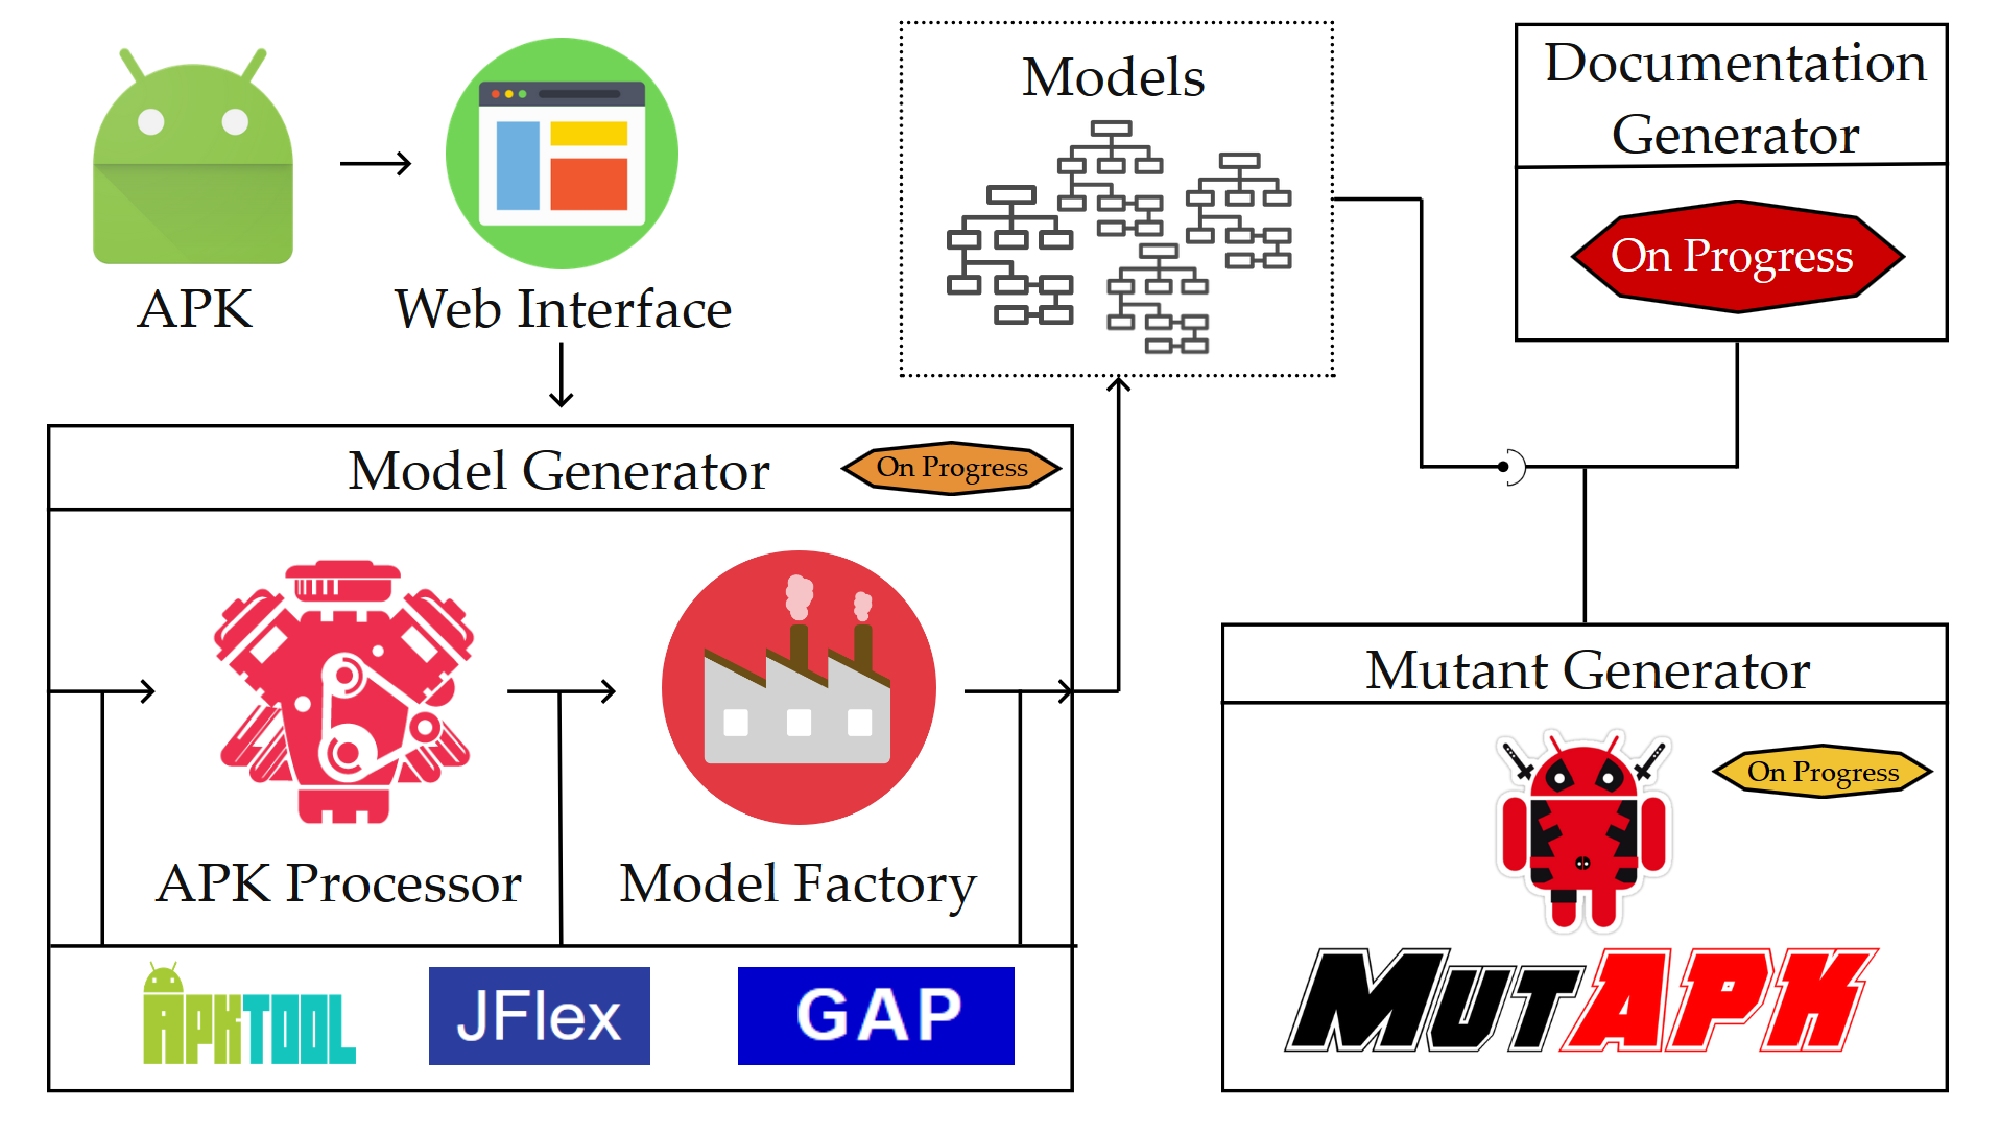
\includegraphics[width=0.9\linewidth]{Figures/Arquitectura}}
%\caption{Proposed Architecture}
%\label{fig}
%\end{figure}
%
%Therefore we present the architecture from the Fig. \ref{fig} that is divide in 4 main sections:
%\subsection*{\textit{\textbf{User Interface}}}
%In order for user to access our tool we present a web interface that will allow to manage the load of an APK, this web interface will be a robust web solution that allows users to: (i) see previous usages of the tool, (ii) access to the models generated for the application and (iii) configure the current usage with the expected results (i.e. on-demand documentation, mutant generation, both of them ).
%
%\subsection*{\textit{\textbf{Model Generator}}}
%Once the user has uploaded the APK the processing task is triggered. This model generator translate the apk into an SMALI representation along with the decoded resources. At this point, it uses a lexer/parser in order to process the SMALI files into a Abstract Sintaxis Tree that will allows the model generator to easily generate other models. At the same time, the model generator process the decoded resources that also provide valuable information as the Android Manifest file, the strings and colors files, creating a representation of the information that can be easily query for further information.
%
%\subsection*{\textit{\textbf{Models storage}}}
%In order to make this tool customizable and extensible we propose that the models generated previously should be stored in a folder where all the extensions tools that enables a software engineering task will search for them. This will allows that other contributors can add other extensions for specific purposes or improve the already created for their needs without worrying of the model generation.
%
%\subsection*{\textit{\textbf{Tool Extensions}}}
%Finally, in order to give real value to the tool, we propose a set of extensions that consumes the models and enables software engineering tasks. For the purpose of this thesis we propose two extensions. The first one is the one in charge of creating documentation for the app. The second one is in charge of creating the mutants for mutation testing.